\actTitle{4.3 - Right Triangle Trigonometry}

\videoLink{Section 4.3}{https://www.youtube.com/playlist?list=PLYHZK3b8UFw2K5Q_epS1Wi1hezUGCYwtP}

\noindent \textbf{Topics:}  acute angles, right triangle trigonometry, cofunction identities\\

\noindent \textbf{Student Learning Outcomes:}
\begin{enumerate}
\item Students will be able to evaluate trigonometric functions of acute angles.
\item Students will be able to use trigonometric identities.
\item Students will be able to use trigonometric functions in applications.
\end{enumerate}

\hrule 

\bigskip

\subsection{Trigonometric Functions of Acute Angles} ~

\noindent An angle is \textbf{\underline{acute}} if it measures less than 90$^{\circ}$.\\
A \textbf{\underline{right angle}} measures exactly 90$^{\circ}$.\\
The sum of angles of a triangle is 180$^{\circ}$.\\[.2in]

\noindent If we know two sides of a right triangle, we can use the
\textbf{Pythagorean Theorem} $a^2+b^2=c^2$ to find the 3rd side.


\begin{center}
  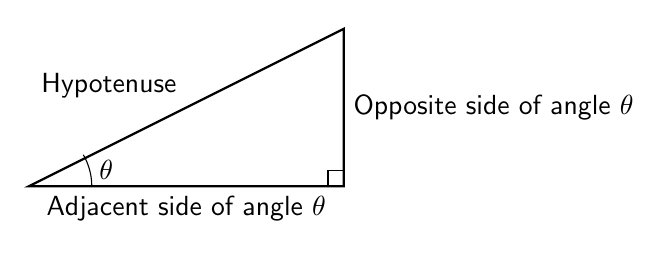
\begin{tikzpicture}[y=1cm, x=1cm,font=\sffamily]
    \draw[black,thick,fill=gray!0] (0,0)--(4,0)--(4,2) -- cycle;
    \draw[black] (3.8,0) -- (3.8,0.2) -- (4,0.2);
    \draw[thin,black] (0.8,0) arc (0:30:0.8)
              node[anchor=west,pos=0.5] {$\theta$};
    \node[anchor=west] at (4,1) {Opposite side of angle $\theta$};
    \node[anchor=north] at (2,0) {Adjacent side of angle $\theta$};
    \node[anchor=south east] at (2,1) {Hypotenuse};
  \end{tikzpicture}
\end{center}

In the \textbf{right} triangle above, the \textbf{\emph{six
    trigonometric functions}} of an angle $\theta$ are defined as
follows:
\begin{eqnarray*}
  \begin{array}{rcl@{\hspace{4em}}rcl@{\hspace{4em}}rcl}
    \sin(\theta) & = & \frac{\textrm{opp.}}{\textrm{hyp.}} & 
    \cos(\theta) & = & \frac{\textrm{adj.}}{\textrm{hyp.}} &
    \tan(\theta) & = & \frac{\textrm{opp.}}{\textrm{adj.}} \\ [10pt]
    \csc(\theta) & = & \frac{\textrm{hyp.}}{\textrm{opp.}} & 
    \sec(\theta) & = & \frac{\textrm{hyp.}}{\textrm{adj.}} &
    \cot(\theta) & = & \frac{\textrm{adj.}}{\textrm{opp.}} 
  \end{array}
\end{eqnarray*}



\newpage





\begin{enumerate}
\item Find the six trig functions of $\theta$ in the triangle below.
  \begin{center}
  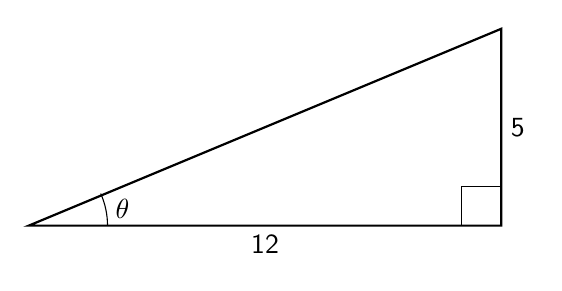
\begin{tikzpicture}[y=0.5cm, x=0.5cm,font=\sffamily]
    \draw[black,thick,fill=gray!0] (0,0)--(12,0)--(12,5) -- cycle;
    \draw[black] (11,0) -- (11,1) -- (12,1);
    \draw[thin,black] (2,0) arc (0:24:2)
              node[anchor=west,pos=0.5] {$\theta$};
    \node[anchor=west] at (12,2.5) {5};
    \node[anchor=north] at (6,0) {12};
  \end{tikzpicture}
\end{center}
\begin{eqnarray*}
  \begin{array}{rcl@{\hspace{4em}}rcl@{\hspace{4em}}rcl}
    \sin(\theta) & = &  & 
    \cos(\theta) & = &  &
    \tan(\theta) & = &  \\ [10pt]
    \csc(\theta) & = &  & 
    \sec(\theta) & = &  &
    \cot(\theta) & = & 
  \end{array}
\end{eqnarray*}

\item Find the sine, cosine, and tangent of 45$^{\circ}$ using the triangle below.

  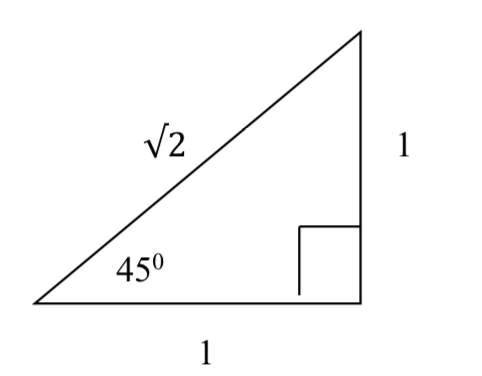
\includegraphics[scale=.6]{trigex2}\\

\item Find the sine, cosine, and tangent of 30$^{\circ}$ and  60$^{\circ}$ using the triangle below.\\
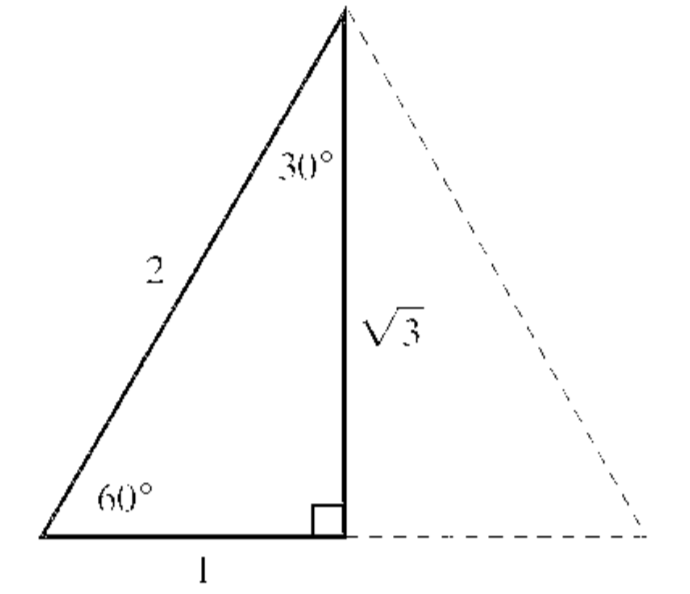
\includegraphics[scale=.6]{trigex3}\\


\newpage

\item Given $\sin(\theta)=\frac{2}{3}$ and $\cos(\theta)=\frac{\sqrt{5}}{3}$, find the value of each of the four remaining functions.\vfill
\vfill


\subsection{Cofunction Identities} ~

\noindent Cofunctions of complementary angles are equal.
$$\sin(\theta)=\cos(90^{\circ}-\theta) \quad \quad \cos(\theta)=\sin(90^{\circ}-\theta)$$
$$\tan(\theta)=\cot(90^{\circ}-\theta) \quad \quad \cot(\theta)=\tan(90^{\circ}-\theta)$$
$$\sec(\theta)=\csc(90^{\circ}-\theta) \quad \quad \csc(\theta)=\sec(90^{\circ}-\theta)$$



\item Fore each function value, find a cofunction with the same value.
\begin{enumerate}
\item $\cot(15^{\circ})=2+\sqrt{3}$\vfill
\item $\displaystyle \cos\Bigg(\frac{\pi}{6}\Bigg)=\frac{\sqrt{3}}{2}$\vfill
\end{enumerate}

\newpage
\subsection{Using Trigonometric Functions in Applications} ~

\item A forester, 300 feet from the base of a redwood tree, observes that the angle between the ground and the top of the tree is 45$^\circ$.  Determine the height of the tree.

\vfill
\item A pilot flying an airplane at an altitude of 1 mile sights a point at the end of a runway.  The angle of depression is 3$^\circ$.  What is the distance $d$ from the plane to the point on the runway?  Round to the nearest tenth of a mile.
\vfill
\vfill
\end{enumerate}

\noindent \textbf{Student Learning Outcomes Check}

\begin{enumerate}
\item Can you evaluate trigonometric functions of acute angles?
\item Are you able to use able to use trigonometric identities?
\item Can you use trigonometric functions in applications?
\end{enumerate}

\noindent \textbf{If any of your answers were no, please ask about these topics in class.}


